\documentclass[tikz]{standalone}
\usetikzlibrary{graphs.standard, shapes.geometric}
\begin{document}
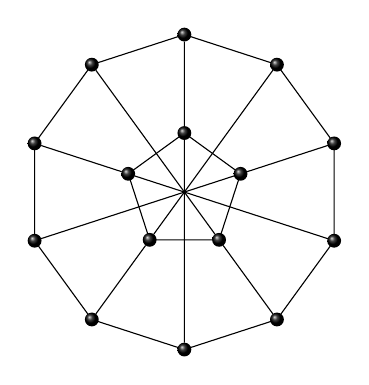
\begin{tikzpicture}[
  rp/.style={regular polygon, regular polygon sides={#1}, outer sep=+0pt},
  ball/.style={
    circle, outer sep=auto, ball color=black, inner sep=0pt, minimum size=5pt}
]
\node[rp=10, minimum size=4cm,   draw=black, rotate=18, name=outer] at (6,6) {};
\node[rp=5,  minimum size=1.5cm, draw=black, name=inner] at (6,6) {};

\foreach \corner in {1,2,...,10}
  \node[ball] (outer-corner-\corner) at (outer.corner \corner){};
\foreach \corner in {1,2,...,5}
  \node[ball] (inner-corner-\corner) at (inner.corner \corner){};

\foreach[evaluate={
  \cOuter=int(2*\cInner-1);
  \cOpposite=int(mod(\cOuter+4,10)+1);
}]\cInner in {1,...,5}
  \draw (outer-corner-\cOuter)
     -- (inner-corner-\cInner)
     -- (outer-corner-\cOpposite);
\end{tikzpicture}

\tikz\graph[
  nodes={
    circle, outer sep=+0pt, ball color=black, inner sep=+0pt, minimum size=+5pt},
  counterclockwise, phase = 90, typeset =,
]{
  subgraph C_n[name=inner, n= 5] -!-
  subgraph C_n[name=outer, n=10],
  { [edge={double=black, red, thick}]
    \foreach[evaluate={
      \cOuter=int(2*\cInner-1);
      \cOpposite=int(mod(\cOuter+4,10)+1);
      }] \cInner in {1,...,5} {
        inner \cInner -- {outer \cOuter, outer \cOpposite}},
  }
};
\end{document}